% -*- root: ../Crypto.tex -*-
\section{Hoja 1}
\begin{problem}[1]
	Un general espartano recibe el siguiente mensaje de un amigo de Cantoblanco:


	SONFAUHPINPEOCTOHRIANEQLSGCUTUOHEEEQOENRUBSETEIDRELEIT

	¿Qué dice el mensaje?

	\solution
	\doneby{Jorge}

	Si consiguiéramos una escítala cuyo diámetro hiciera que entraran 5 letras por fila conseguiríamos el mensaje:

	SUPONGOQUELOHEHECHOBIENPORQUEESDIFICILTENERTANTASUERTE

\end{problem}

\begin{problem}[2]
	Recibes el mensaje VEILRÑW, cifrado usando una clave de Cesar en el alfabeto castellano de 27 letras (con Ñ y W). Lee el mensaje, da las transformaciones para cifrar y descifrar, y cifra el mensaje GRACIAS utilizando la clave correspondiente.

	\solution
	\doneby{Jorge}

	Usando la transformación:
	\[\appl{f_{17}}{ℤ/27}{ℤ/27}\]
	\[f_{17}(x) = x + 17\]

	Se consigue $f_{17}(\{V,E,I,L,R,Ñ,W\}) = \{M,U,Y,B,I,E,N\}$.

	De modo que para cifrar nos basta:
	\[f_{17}^{-1}(x) = f_{-17}(x) = f_{10}(x)\]
	\[f_{10}(\{G,R,A,C,I,A,S\}) = \{P,B,K,M,R,K,C\}\]
\end{problem}

\begin{problem}[3]
	Utilizando el análisis de frecuencias, descifra el siguiente mensaje, del que sabes que está escrito en inglés (26 letras, con W pero sin Ñ) y que ha sido cifrado con una clave de Cesar:
	PXPXKXENVDRUXVTNLXHYMXGMAXYKXJNXGVRFXMAHWGXXWLEHGZXKVBIAXKMXQM

	\solution
	\doneby{Jorge}

	Al hacer el análisis de frecuencias se obtiene:

	\begin{center}
		\begin{tabular}{ l l }
			P & 0.03225806451612903 \\
			X & 0.24193548387096775 \\
			K & 0.06451612903225806 \\
			E & 0.03225806451612903 \\
			N & 0.04838709677419355 \\
			V & 0.06451612903225806 \\
			D & 0.016129032258064516 \\
			R & 0.03225806451612903 \\
			U & 0.016129032258064516 \\
			T & 0.016129032258064516 \\
			L & 0.03225806451612903 \\
			H & 0.04838709677419355 \\
			Y & 0.03225806451612903 \\
			M & 0.08064516129032258 \\
			G & 0.06451612903225806 \\
			A & 0.04838709677419355 \\
			J & 0.016129032258064516 \\
			F & 0.016129032258064516 \\
			W & 0.03225806451612903 \\
			Z & 0.016129032258064516 \\
			B & 0.016129032258064516 \\
			I & 0.016129032258064516 \\
			Q & 0.016129032258064516
		\end{tabular}
	\end{center}

	Se puede ver que la más frecuente entre todas es la letra X. Si tomamos como letra más usada del ingés la E (en vez de la T) se obtiene el mensaje:

	WEWERELUCKYBECAUSEOFTENTHEFREQUENCYMETHODNEEDSLONGERCIPHERTEXT

	Gracias a la transformación $f_{7}(x) = x + 7$.
\end{problem}

\begin{problem}[4]
	La distribución de frecuencias (en porcentaje) en castellano de las 26 letras (es decir, sin W) es aproximadamente la siguiente.

	\begin{tabular}{c c c c c c c c c c c c c c c c c c c c c c c c c c c}
		A & B & C & D & E & F & G & H & I & J & K & L & M \\
		12,6 & 1,0 & 5,1 & 5,7 & 13,7 & 0,9 & 0,8 & 0,5 & 7,0 & 0,2 & 0,0 & 4,6 & 3,2 \\
		N & Ñ & O & P & Q & R & S & T & U & V & X & Y & Z \\
		7,0 & 0,1 & 8,8 & 2,9 & 1,1 & 6,6 & 7,2 & 5,1 & 3,9 & 0,8 & 0,1 & 0,6 & 0,3
	\end{tabular}

	Recibes un mensaje escrito en castellano (con ese alfabeto) que ha sido cifrado con el criptosistema de Cesar. Las dos letras más frecuentes en el texto cifrado son, por ese orden, la J y la N. Deduce razonadamente cual puede haber sido la clave utilizada para cifrar.

	\solution
	\doneby{Jorge}

	Lo lógico sería que las letras más frecuentes en el alfabeto se correspondieran con las más correspondientes en el mensaje, de modo que lo primero que a uno se le viene a la cabeza es corresponder la J (la más frecuente en el mensaje) con la E (la más frecuente en el alfabeto). Esto viene a ser la transformación $f_{-5}=f_{21}$, la cual manda la N (la segunda más frecuente en el mensaje) a la I (que no es la segunda más frecuente en el español).

	De modo que igual la segunda más frecuente en el mensaje es la que se corresponde con la más frecuente en el alfabeto ($f_{-9}=f_{17}$). Con esta transformación se consigue:
	\[f_{17}(J)=A\]
	\[f_{17}(N)=E\]
	Lo cual es más coherente, ya que hace una correspondencia entre las 2 letras más frecuentes del alfabeto (la E y la A) con las 2 más frecuentes del mensaje.
\end{problem}

\begin{problem}[5]
	Interceptamos un mensaje en el que dos profesores hablan de las asignaturas del plan de estudios de Matemáticas. El mensaje es el siguiente:

	DONQONHOSDGXQKCHDKSNSJSDOQOBDCUQ

	Sabemos que el mensaje ha sido cifrado utilizando una sustitución simple en el alfabeto castellano de 27 letras (con Ñ y W), y sospechamos que en el mensaje original aparecía la palabra CALCULO. Lee el mensaje.

	\solution
	\doneby{Jorge}

	Haciendo el análisis de frecuencias del mensaje interceptado se obtiene:

	\begin{center}
		\begin{tabular}{l l}
			D & 0.15625 \\
			O & 0.15625 \\
			N & 0.09375 \\
			Q & 0.125 \\
			H & 0.0625 \\
			S & 0.125 \\
			G & 0.03125 \\
			X & 0.03125 \\
			K & 0.0625 \\
			C & 0.0625 \\
			J & 0.03125 \\
			B & 0.03125 \\
			U & 0.03125
		\end{tabular}
	\end{center}

	Dentro del mensaje interceptado CALCULO se corresponde con NQONHOS, para darse cuenta basta con fijarse que hayan dos pares de letras iguales al igual que pasa en CALCULO. Con dicha correspondencia de letras tenemos (mostramos el mensaje cortado en 2, donde la fila de debajo de cada trozo se corresponde con lo que llevamos descifrado):

	\begin{center}
		\begin{tabular}{c c c c c c c c c c c c c c c c}
			D & O & N & Q & O & N & H & O & S & D & G & X & Q & K & C & H \\
			\_ & L & C & A & L & C & U & L & O & \_ & \_ & \_ & A & \_ & \_ & U
		\end{tabular}
	\end{center}

	\begin{center}
		\begin{tabular}{c c c c c c c c c c c c c c c c}
			D & K & S & N & S & J & S & D & O & Q & O & B & D & C & U & Q \\
			\_ & \_ & O & \_ & O & \_ & O & \_ & L & A & L & \_ & \_ & \_ & \_ & A
		\end{tabular}
	\end{center}

	Puesto que el análisis de frecuencias nos dice que la D es la letra que más aparece, probaremos a corresponderla con la letra E:

	\begin{center}
		\begin{tabular}{c c c c c c c c c c c c c c c c}
			D & O & N & Q & O & N & H & O & S & D & G & X & Q & K & C & H \\
			E & L & C & A & L & C & U & L & O & E & \_ & \_ & A & \_ & \_ & U
		\end{tabular}
	\end{center}

	\begin{center}
		\begin{tabular}{c c c c c c c c c c c c c c c c}
			D & K & S & N & S & J & S & D & O & Q & O & B & D & C & U & Q \\
			E & \_ & O & \_ & O & \_ & O & E & L & A & L & \_ & E & \_ & \_ & A
		\end{tabular}
	\end{center}

	Fijándonos en que la K y la C son las siguientes letras con mayor frecuencia, y que de entre las no utilizadas del alfabeto, la S y N son las siguientes que tienen más frecuencia en español. Probando se llega a que la K va a la N, y la C a la B.

	\begin{center}
		\begin{tabular}{c c c c c c c c c c c c c c c c}
			D & O & N & Q & O & N & H & O & S & D & G & X & Q & K & C & H \\
			E & L & C & A & L & C & U & L & O & E & \_ & \_ & A & N & B & U
		\end{tabular}
	\end{center}

	\begin{center}
		\begin{tabular}{c c c c c c c c c c c c c c c c}
			D & K & S & N & S & J & S & D & O & Q & O & B & D & C & U & Q \\
			E & N & O & \_ & O & \_ & O & E & L & A & L & \_ & E & B & \_ & A
		\end{tabular}
	\end{center}

	Llegados a este punto, somos capaces de adivinar que lo que pone el mensaje es:

	EL CALCULO ES TAN BUENO COMO EL ALGEBRA
\end{problem}


\begin{problem}[6]
	Interceptamos cuatro mensajes cifrados. Sabemos que tanto los mensajes en claro como los mensajes cifrados han sido escritos utilizando el alfabeto inglés de 26 letras. Las frecuencias con que cada letra aparece en cada mensaje son las siguientes:

	\begin{center}
		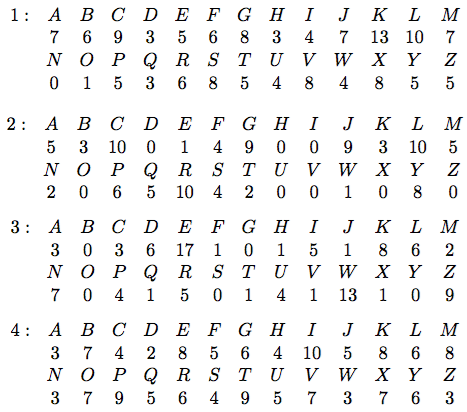
\includegraphics[width=0.5\textwidth]{img/freqsEj1_6}
	\end{center}

	¿Cuáles de los mensajes es razonable pensar que han sido cifrados utilizando sustituciones simples sobre letras?

	\solution
	\doneby{Pedro}

	Lo único que podemos hacer es fijarnos en las frecuencias de las diferentes letras y ver en qué mensajes las letras tienen unas frecuencias similares a las del inglés.

	Basándonos en la tabla de frecuencias de moodle podemos agrupar las letras del alfabeto inglés según la frecuencia con que se usan (en inglés y en cada uno de los mensajes interceptados).

	Si la columna de un mensaje se asemeja a la segunda columna, ese mensaje tendrá alta probabilidad de haber sido cifrado empleando una sustitución simple sobre letras.

	\begin{center}
	\begin{tabular}{| c | c || c | c | c | c |}
	\hline
	\textbf{Porcentaje} & \textbf{Nº Ingles} & \textbf{Nº M1} & \textbf{Nº M2} & \textbf{Nº M3} & \textbf{Nº M4} \\
	\hline
	0-2 & 10 & 2 & 9 & 12 & 0\\
	\hline
	2-4 & 6 & 3 & 4 & 3 & 5 \\
	\hline
	4-6 & 1 & 8 & 5 & 3 & 7 \\
	\hline
	6-8 & 7 & 6 & 1 & 3 & 8 \\
	\hline
	8-10 & 1 & 5 & 3 & 2 & 5 \\
	\hline
	>10 & 1 & 2 & 3 & 2 & 1 \\
	\hline
	\end{tabular}
	\end{center}

	Antes de nada hay que comentar que no sabemos qué longitud tenía cada mensaje por lo que tampoco sabemos cómo de válidas son las frecuencias calculadas. Por ello se ha tomado la decisión de agrupar las frecuencias por valores.

	Si sabemos que cada mensaje era un ``Los Pilares de la Tierra'' en inglés y cifrado, tendremos unas estimaciones de la frecuencia de cada letra muy muy buenas, por lo que podríamos agrupar las frecuencias por unidades.

	El primer y el último mensajes tienen muy pocas letras con baja frecuencia y demasiadas con frecuencia 8-10 por lo que parece razonable descartar la posibilidad de que hayan sido escritos en inglés.

	Entre el segundo y el tercero, el que más posibilidades tiene de haber sido escrito originalmente en inglés es el tercero, pues el segundo tiene muy pocas letras con frecuencia 6-8 y quizás demasiadas con frecuencias altas.

	Para el espía experto otra posibilidad sería estudiar la media y la varianza de la distribución de frecuencias en cada mensaje y apoyarse también en eso a la hora de tomar la decisión.
\end{problem}


\begin{problem}[7]
	En un alfabeto de 28 letras, las 27 del castellano y el espacio=27, utiliza la clave afíın sobre letras $f(m) = 13m + 9$ para cifrar el mensaje ``MUY BIEN''.

	\solution

	\doneby{Jorge}

	Utilizamos el $\_$ para representar el espacio y que este se vea claro.
	\[f(``MUY\_BIEN'')=``SXTRPW\_E''\]
\end{problem}


\begin{problem}[8]
	Sabemos que el enemigo está utilizando transformaciones afines sobre letras para cifrar mensajes escritos en inglés con el siguiente alfabeto de 37 letras: los números 0,...,9 que se codifican como ellos mismos; las letras A,…,Z (con W, sin Ñ), que corresponden a 10,…,35; y el espacio en blanco=36. Interceptamos el siguiente mensaje cifrado

	OH7F86BB46R3627O266BB9 (Atención, no hay ceros, sólo os)

	Sabiendo que el mensaje original acaba con la firma 007 (cero, cero, siete), ¿qué dice el mensaje?

	\solution
	\doneby{Jorge}

	La transformación afín será de la forma:
	\[ f_{a,b}(x) = ax+b \]

	Luego planteando un sistema de ecuaciones obtenemos a y b, sabemos que B=11:
	\[ f_{a,b}(11) = a·11 + b = 0\]
	\[ f_{a,b}(9)  = a·9  + b = 7 \]

	\[ b = -11a = 26a \]

	Luego
	\[ 9a + 26a = 35a = 7 \implies a = 15  \implies b = 20\]

	Aplicando $f_{a,b}$ al mensaje cifrado se obtiene:
	\begin{center}
		``AGENT 006 IS DEAD  007''
	\end{center}
\end{problem}


\begin{problem}[9]
	Una unidad de texto (en claro) m se dice que es fija para una transformación para cifrar si $f(m) = m$. Supongamos que estamos usando transformaciones afines sobre letras en un alfabeto de N letras, $f(m) = a · m + b$ con $a ≠ 1$.

	\begin{enumerate}
		\item Demostrar que si N es primo hay exactamente una letra fija.
		\item Demostrar que para N arbitrario cualquier transformación lineal (es decir, con b = 0) tiene al menos una letra fija, y que si N es par cualquier transformación lineal tiene al menos dos letras fijas.
		\item Dar un ejemplo de una transformación afín (para algún N) sin letras fijas.
	\end{enumerate}

	\solution
	\doneby{Jorge}
	\begin{enumerate}
		\item $m = a · m + b  \implies (a-1)·m + b = 0 \implies m = -(a-1)^{-1} · b$. En caso de que $N$ sea primo sabemos que existe $(a-1)^{-1}$, ya que en ese caso $U(ℤ/N)=ℤ/N$ y por tanto $(a-1) ∈ U(ℤ/N)$. Así que $m$ es único al quedar determinado por el producto de $(a-1)^{-1}$ y $b$.

		\item En caso de que $f(m) = a·m$ sabemos que siempre tendremos la letra fija asociada al 0 (ya que $f(0)=0$) independientemente de qué $N$ tengamos.

		Si $f(m) = a·m$ con $N$ par ($N=2M$), se cumple, además, que $f(M)=M$, ya que

		\[f(M)=M \iff aM = M \iff (a-1)M = 0 \iff 2M | (a-1)M \]

		Y puesto que $a$ debe ser unidad en $\ent_{2M}$, debe ser coprimo con $2M$ y, por tanto, impar. Por tanto, es claro que $(a-1)$ será par y, efectivamente $(a-1)M = k \cdot 2M$

		\item Para $N=2$ la transformación $f(x) = x + 1$ no deja letras fijas.
	\end{enumerate}
\end{problem}

\begin{problem}[10]
	Sea $A$ un anillo conmutativo con 1. Diremos que $a∈A$ es un divisor de 0 si existe $b∈A$, $b≠0$ y tal que $ab = 0$ (con esta definición, que no es la normal, 0 es un divisor de 0, pero no importa, simplifica los enunciados). Diremos que $a ∈ A$ es una unidad si existe $b ∈ A$ tal que $ab = 1$.

	\ppart Demostrar que $\left\{ \text{Unidades de } A \right\} ∩ \left\{ \text{Divisores de 0 en } A \right\} = \emptyset$
	\ppart Dado $a ∈ A$, definimos la aplicación ``multiplicar por $a$'', $\appl{m_a}{A}{A}$ como $m_a(x) = ax$. Caracterizar los divisores de 0 (o quizá los no divisores de 0) y las unidades de $A$ en términos de propiedades de la correspondiente aplicación $m_a$.
	\ppart Utilizar la caracterización anterior para demostrar que si $A$ es un anillo finito se tiene:

		\[\left\{ \text{Unidades de } A \right\} \cup \left\{ \text{Divisidores de 0 en } A \right\} = A\]

		(Esto generaliza lo que sucede en los anillos de congruencias $ℤ/Nℤ$.)
	\ppart Demostrar que la hipótesis de finitud es esencial en el apartado 3.

	\solution
	\doneby{Pedro}

	\spart
	Supongamos que tenemos un elemento $x$ que es unidad y divisor de 0 simultáneamente.

	En ese caso tendríamos que existen dos números $a$ y $b$, ambos distintos de 0, tales que: $ax = 0$ y $bx = 1$

	En esta situación podemos tomar la ecuación $bx=1$ y multiplicar por $a$ a ambos lados, con lo que mantenemos la igualdad, obteniendo:
	\[bx = 1 \iff abx = a \iff axb = a \iff 0 \cdot b = a \iff 0 = a\]

	Con lo que llegamos a una contradicción, pues dijimos que $a \neq 0$

	\spart

	Si tenemos que $a$ es un divisor de 0, habrá algún valor (distinto de 0) que nos llevará a 0, con lo que la función $f_a$ no será inyectiva.

	A raíz de esto podemos ver que si $a$ no es un divisor de 0, la función $m_a(x)=ax$ será inyectiva. Para comprobarlo basta con ver que:
	\[\forall x\neq y, \ ax=ay \implies a(x-y)=0 \implies a \text{ divisor de 0 ya que } x-y \neq 0\]
	lo que nos lleva a una contradicción.

	Por otro lado, si $a$ es una unidad, la función será sobreyectiva pues tendremos:
	\[\forall y \ ax = y \implies x = ya^{-1} \implies \exists x \tq m_a(x)=y\]

	Además, de esta misma fórmula podemos deducir que si no es unidad, no será sobreyectiva la función (no podremos llegar al 1, por ejemplo)

	\spart

	Si tenemos un elemento $a \in A$ que no es unidad ni divisor de 0 en $A$, tendremos que la función asociada $m_a$ será inyectiva pero no sobreyectiva.

	Si una función entre dos conjuntos finitos es inyectiva pero no sobreyectiva, esto implica que el conjunto de partida es menor que el de llegada. Pero por definición, la función $m_a$ va de un conjunto en si mismo, con lo que es imposible que sea inyectiva y no sobreyectiva.

	Por tanto es imposible que exista un $a$ como el que hemos definido. Es decir, tenemos demostrado que
	\[\left\{ \text{Unidades de } A \right\} \cup \left\{ \text{Divisidores de 0 en } A \right\} \supset A\]

	El otro sentido del contenido es trivial por la propia construcción del conjunto de unidades y de los divisores.

	\spart

	Si $A$ se tratase del anillo $(\ent, +, \cdot )$, dado $a=2$ podemos construir una aplicación $m_a$ que, como se probó en el apartado anterior, sería inyectiva pues 2 no es divisor de 0.

	Sin embargo, al no ser un cuerpo finito no hay problema en que una función vaya de un anillo en si mismo siendo inyectiva pero no sobreyectiva. Por tanto no podríamos deducir ninguna relación de contención.

	\doneby{Edu}

	\spart[a]

	Supongamos x $\in \text{Unidades de } A$ y $\exists y \neq 0 \tq x\cdot y = 0$, ie, x $\in \text{Divisores de 0 en } A$:
	\[ x \cdot y = 0 \implies x^{-1} \cdot x \cdot y = 0 \implies y = 0 \Rightarrow \Leftarrow \]
	{\bf Conclusión:} si x $\in \text{Unidades de } A \implies$ x $\not\in \text{Divisores de 0 en } A$

	Supongamos x $\in \text{Divisores de 0 en } A$, ie, $\exists y \neq 0 \tq x \cdot y = 0$ y supongamos $\exists z \neq 0 \tq x \cdot z = 1$:
	\[ x \cdot z = 1 \implies y \cdot x \cdot z = y \cdot 1 \implies 0 \cdot z = y \implies 0 = y \Rightarrow \Leftarrow \]
	{\bf Conclusión:} si x $\in \text{Divisores de 0 en } A  \implies$ x $\not\in \text{Unidades de } A$
	\newline\qed

	\spart[b]

	Si $m_a$ es inyectiva (y {\bf por ser A finito} entonces es sobreyectiva)

	$\implies \forall x,y \neq 0 \in A$, $m_a(x) = xa = ya = m_a(y) \implies x = y \implies $ a $\in $ unidades de A ya que, al ser {\bf sobreyectiva}, $\exists y \in A \tq a\cdot y = 1$.

	Si $m_a$ no es sobreyectiva, ie, GCD($m\cdot a$, |A|) $> 1$ para algún a, $\exists x,y \in A, x \neq y \tq$ $a \cdot x = a \cdot y \implies a (x - y) = 0 \implies a$ es divisor de 0.

	\spart[c]

	Como observación, diremos que si la afirmación es falsa, por el apartado 1, tiene que existir un $x$ que no pertenece a ninguno de los dos subconjuntos de A, lo cual es imposible por el apartado anterior: si $m_a$ es inyectiva, entonces $a$ es unidad, si $m_a$ no es sobreyectiva, $a$ es divisor de 0.
\newline\qed

	\spart[d]

	Leer la parte negrita del apartado B y convencerse de que no tiene por qué existir el inverso de $a$.

\end{problem}





\section{Control 1 (22-09-2014) Modelo A}
\begin{problem}[1]
Dado $N\geq 2$ y un elemento $a \in \ent_N$, consideramos la aplicación $\appl{m_a}{\ent_N}{\ent_N}$ tal que $m(x)=ax$.

Demostrar que son equivalentes:
\begin{enumerate}
\item $a$ es unidad en $\ent_N$
\item $a$ y $N$ son primos entre si.
\item $m_a$ es inyectiva
\item $m_a$ es sobreyectiva
\end{enumerate}

\solution
\doneby{Pedro}

Para demostrar que los enunciados son equivalentes vamos a demostrar una serie de implicaciones de modo que, al final, desde cualquiera de esas afirmaciones podamos llegar a cuaquier otra.

\begin{itemize}
\item \textbf{$1 \implies 2$}
Si $a$ es una unidad en $\ent_N$ sabemos que existe $c \in \ent_N$ tal que
\[ac = kN + 1\]

Supongamos ahora que $a$ y $N$ no son primos entre si, es decir,
\[\exists b \tq a = b \cdot a' \text{ y } N = b \cdot N'\]

Sustituyendo en la primera fórmula obtenemos
\[ba'c=bkN'+1 \iff b(a'c-kN')=1 \iff b \in U(\ent_N)\]

Pero está claro que $b$ no puede pertenecer a las unidades de $\ent_N$ ya que, siempre que $bc< N$ es claro que $bc \neq 1$ salvo que ambos sean 1 y, además:
\[\forall c \in \ent_N, \tq cb > N \iff cb = bN'α+bβ \text{ siendo } bβ < N\]
con lo que el resto nunca será 1.

\item \textbf{$2 \implies 3$}

Ahora tenemos $a$, $N$ tales que $(a,N)=1$ y queremos ver que la función $m_a$ es inyectiva.

Suponemos que no es inyectiva y que por tanto $\exists x,y \in \ent_N$ tales que $x \neq y$ y:
\[ax=ay \text{ mod } n \iff a(x-y)= 0 \ \text{mod } n \iff a(x-y) = c N\]

Pero, en caso de ser esto cierto, por definición, $a$ sería un divisor de $cN$ y, por tanto, $a$ divide a $c$ ya que estamos considerando $(a,N)=1$.

Si $a$ fuese divisor de $c$, podríamos escribir:
\[a(x-y)=kaN \iff (x-y) = kN\]
pero consideramos que $x$ y $y$ son dos elementos distintos de $\ent_N$ y, por tanto, su diferencia no puede ser múltiplo de $N$. Con lo que llegamos a una contradicción.

Por tanto no pueden existir $x$, $y$ como los descritos con lo que queda claro que la función es inyectiva.

\item \textbf{$3 \implies 4$}
Como estamos moviéndonos en un conjunto finito, si la función es inyectiva debe ser también sobreyectiva.

\item \textbf{$4 \implies 1$}

Si la función es sobreyectiva, entonces
\[\forall c \in \ent_N \exists b \in \ent_N \tq ab=c\]
en concreto esto es cierto para $c=1$ y por tanto $a$ tiene inverso, es decir, pertenece a las unidades de $\ent_N$

\end{itemize}

\end{problem}

\begin{problem}[2]
En un idioma que se escribe usando el mismo alfabeto que el inglés (26 letras), las letras más frecuentes son $B(20\%)$ y $Z(13\%)$, sin que ninguna de las demás letras tenga una frecuencia superior al $5\%$

Interceptamos un texto escrito en este idioma que ha sido cifrado usando un criptosistema afín sobre las letras vistas como elementos de $\ent_{26}$. Las letras más frecuentes en el mensaje cifrado resultan ser, por este orden, $H$ y $D$.

¿Qué letra en claro dirías que corresponde con la $E$ cifrada?

\solution
\doneby{Pedro}

Vamos a calcular directamente la función de descifrado, que será de la forma $f(m)=αm+β$. Sustituyendo los datos que tenemos nos queda el sistema:
\[\left\{
7α +β  = 1 \atop
3α + β = 25
\right. \implies 22α = 24 \implies 11α = 12 \]

Para resolver la ecuación tenemos que calcular el inverso de $11$ módulo 26. Para ello aplicamos el algoritmo de Euclides:
\[\begin{array}{l}
26 = 2 \cdot 11 +4\\
11 = 2 \cdot 4+ 3\\
4 = 1 \cdot 3 + 1
\end{array} \implies \begin{array}{l}
1 = 4 - 3 \\
3 = 11 - 2 \cdot 4 \implies 1 = 4 - 11 + 2 \cdot 4 = 3\cdot 4 -11 \\
4 = 26 -2 \cdot 11 \implies 1 = 3 \cdot 26 -6\cdot 11 - 11 = 3 \cdot 26 -7\cdot 11
\end{array}\]

Finalmente tenemos que $1 = 3\cdot 26 + 19 \cdot 11$, con lo que podemos resolver la ecuación, pues
\[α = 19 \cdot 12 = 20 \implies β = 17\]

Ahora podemos descifrar la letra $E$ obteniendo:
\[f(E)=f(4) = 15 = P\]
\end{problem}


\section{Hoja 2}
\begin{problem}[1]
El enemigo escribe en inglés y, para cifrar sus mensajes, utiliza transformaciones afines sobre digrafos en el siguiente alfabeto de 30 letras: las letras A,...,Z (con W, sin Ñ) corresponden a 0,...,25; el espacio=26; ?=27; !=28; ’=29. Interceptamos el siguiente mensaje cifrado:
\begin{center}
DXM SCE DCCUVGX
\end{center}

Un análisis de frecuencias sobre texto interceptado con anterioridad muestra que los digrafos más frecuentes son, por este orden, “M ”, “U ” e “IH”.

En inglés escrito con este alfabeto los digrafos más frecuentes son, por orden, “E ”, “S ” y “ T”.
\ppart Encuentra la clave para descifrar y lee el mensaje.
\ppart Encuentra la clave para cifrar y encripta el mensaje YES I’M JOKING!

\solution

\doneby{Pedro}

\spart
La función que emplearemos para descifrar el mensaje será de la forma: $f(m)=αm+β$ siendo α una matriz 2x2.

Así podemos plantear el sistema de ecuaciones:
\[
\left\{
386α+β = 146 \atop
626α+β = 566
\right. \implies 240α = 420\]

Ahora debemos calcular el inverso de 240 módulo $30 ^2 = 900$ pero 240 no es coprimo con 900 por lo que no será invertible.

Vamos a emplear el tercer par de letras más frecuentes para intentar plantear un sistema que podamos resolver. Así llegamos a
\[
\left\{
386α+β = 146 \atop
247α +β = 799
\right. \implies 761α = 653\]

Empleamos ahora el algoritmo de euclides para calcular el inverso de 761 en $\ent_{900}$
\[\begin{array}{l}
900 = 761 + 139\\
761 = 5\cdot 139 + 66 \\
139 = 2 \cdot 66 + 7\\
66 = 9\cdot 7 + 3 \\
7 = 2 \cdot 3 + 1
\end{array} \implies \begin{array}{l}
1 = 7 - 2 \cdot 3 \\
3 = 66 - 9 \cdot 7 \implies 1 = 19 \cdot 7 -2 \cdot 66 \\
7 = 139 - 2 \cdot 66 \implies 1 = 19 \cdot 139 -40 \cdot 66 \\
66 = 761 - 5 \cdot 139 \implies 1 = -40 \cdot 761 +219 \cdot 139 \\
139 = 900-761 \implies 1 = 219 \cdot 900 -259 \cdot 761
\end{array}\]

Así tenemos que el inverso de 761 es -259 = 641 con lo que podemos calcular
\[α = 641 \cdot  653 = 73 \implies β = 768\]

Ahora podemos descifrar el mensaje llegando a:
\begin{center}
ARE YOU JOKING?
\end{center}

\spart

En esta ocasión debemos resolver el sistema de ecuaciones:

\[
\left\{
146α+β = 386 \atop
799α +β = 247
\right. \implies 653α = 761\]

Empleamos ahora el algoritmo de Euclides para calcular el inverso de 653.
\[\begin{array}{l}
900 = 653 + 247\\
653 = 2\cdot 247 + 159\\
247 = 159 + 88\\
159 = 88 + 71\\
88 = 71 + 17 \\
71 = 4 \cdot 17 + 3 \\
17 =5 \cdot 3 + 2 \\
3 = 2 + 1
\end{array} \implies \begin{array}{l}
1 = 3 - 2 \\
2 = 17 - 5 \cdot 3 \implies 1 = 6 \cdot 3 - 17\\
3 = 71 - 4 \cdot 17 \implies 1 = 6 \cdot 71 -25\cdot 17 \\
17 = 88 - 71 \implies 1 =-25 \cdot 88 +31 \cdot 71 \\
71 = 159 -88 \implies 1 = 31 \cdot 159 -56 \cdot 88 \\
88 = 247 - 159 \implies 1 = -56 \cdot 247 +87 \cdot 159\\
159 = 653 - 2 \cdot 247 \implies 1 = 87 \cdot 653 -230\cdot 247 \\
247 = 900 - 653 \implies 1 = -230 \cdot 900 + 317 \cdot 653
\end{array}\]

Ṕor tanto el inverso de 653 es 317. Gracias a ello podemos calcular
\[α = 317 \cdot 761 = 37 \implies β = 384\]

Por último, solo nos queda cifrar el mensaje usando esta función, con lo que obtenemos
\begin{center}
VQKCAVICN MIQM
\end{center}

\doneby{Jorge}

Si la función de descifrado del aptdo. (a) es:
\[f(c) = α·c + β = m\]
Tendremos que la de cifrado será:
\[f^{-1}(m) = α^{-1}m-α^{-1}β = c\]

Echando cuentas (las he hecho con el ordenador :) ) se llega al mismo resultado que Pedro.

\end{problem}

\begin{problem}[2]
Ciframos un mensaje utilizando una transformación afín sobre n-grafos en un alfabeto de $N$ letras vistos como elementos de $\ent_{N^n}$. Escribimos el texto original como $m_1m_2m_3...$ y el cifrado como $c_1c_2c_3...$, donde cada $m_i$, $c_i$ es una letra.

\ppart Demuestra que $c_{in}$ depende sólo de $m_{in}$, esto es, que cada n-ésima letra cifrada depende sólo de la correspondiente letra sin cifrar.

\ppart Utiliza la observación anterior para explicar cómo alguien que intercepte el mensaje, que sepa que la clave es afín en n-grafos, pero que desconozca n, puede utilizar el índice de coincidencia para averiguar la longitud de la clave.

\solution

\doneby{Pedro}

\spart
Cuando ciframos un mensaje agrupamos las letras a cifrar en bloques, en este caso de longitud $n$. Es evidente que $c_i$ no dependerá de aquellas $m_j$ que no pertenezcan al bloque cifrado.

Supongamos que ciframos las letras $m_1,...,m_n$. En este caso, la relación entre las letras sin cifrar y las cifradas queda representada por la ecuación:
\[α\sum_{i=1}^n m_i\cdot N^{n-i} + β= \sum_{i=1}^n c_i\cdot N^{n-i}\ \text{ mod } N^n\]

Pero la única posibilidad de que esas ecuaciones coincidan es que $α\cdot m_i=c_i, \ \forall i \neq N$ y $αm_N +β = c_N$.

\begin{remark}
En el fondo estamos escribiendo números en formato $n-ario$. La única forma de que dos números en la misma base sean iguales es que los coeficientes sean iguales. Véase los casos a los que estamos acostumbrados como base 10 o base 2.
\end{remark}

\doneby{Jorge}

Sabemos que la cadena de letras $m_1m_2…m_n$ la codificamos como $N^{n-1}m_1 + N^{n-2}m_2 + … + Nm_{n-1} + m_n = \sum_{i=1}^n N^{n-i}m_i$.

De modo que al pasar una cadena de este tipo por una función afín nos queda:
\[c_1…c_n = f(m_1…m_n) = f\left(N^n \sum_{i=1}^n N^{-i} m_i\right) = αN^n \sum_{i=0}^nN^{-i}m_i + β\]

Puesto que estamos en $ℤ_{N^n}$ tendremos (escribiendo también la secuencia codificada en forma de suma):
\[α \sum_{i=0}^n N^{-i}m_i + β = \sum_{i=0}^n N^{-i}c_i\]

Expresando $β$ en forma de suma $β = \sum_{i=0}^n N^{-i}β_i$ :
\[\sum_{i=0}^n N^{-i}(α m_i + β_i) = \sum_{i=0}^n N^{-i}c_i\]

Para el caso particular $n=1$ se tiene que $αm_1 + β_1 = c_1$, y se ve que $c_1$ es función afín de $m_1$. Procediendo por \textbf{inducción} llegamos a que cada $c_i$ es función afín del $m_i$ correspondiente.


\spart
Puesto que cada letra depende únicamente de la letra que ocupa su misma posición en el menaje original, nos encontramos ante la misma situación que en \textbf{Criptosistema de Vigenère} visto en clase y, de la misma forma, podríamos apoyarnos en el \textbf{índice de coincidencia} para encontrar $N$.
\end{problem}

\begin{problem}[3]
Interceptas el mensaje, escrito en inglés, ``!IWGVIEX!ZRADRYD'' que se ha cifrado usando una transformación lineal sobre vecores de $\ent_{29}^2$, donde los números del 0 al 25 equivalen a las letras de la A a la Z, el espacio es el 26, 27 = ? y 28 = !. Sabemos que la súltimas 5 letras del mensaje son la firma, MARIA.

\ppart Descifra el mensaje

\ppart Encuentra la matriz para cifrar y, haciéndote pasar por JO, que es la amiga a quien escribía María, envía cifrado el siguiente mensaje: ``DAMN FOG! JO''


\solution
\doneby{Jorge}

\approvedby{Carolina}

\spart
Nos serviremos de que ADRYD es la codificación de MARIA, y de que el mensaje se cifra a pares. De modo que para obtener la matriz $A$ para decodificar usaremos que $f(DR)=AR$ y $f(YD)=IA$.

\[ \left( \begin{array}{cc}
	a & b \\
	c & d
	\end{array} \right)
	%
	\left( \begin{array}{cc}
	3 \\
	17
	\end{array} \right)
	=
	\left( \begin{array}{cc}
	0 \\
	17
	\end{array} \right)
\]
\[
	\left( \begin{array}{cc}
	a & b \\
	c & d
	\end{array} \right)
	%
	\left( \begin{array}{cc}
	24 \\
	3
	\end{array} \right)
	=
	\left( \begin{array}{cc}
	8 \\
	0
	\end{array} \right)
\]

De estas matrices obtenemos los dos sistemas de ecuaciones:
\[
  \begin{cases}
    3a + 17b = 0\\
    24a + 3b = 8\\
  \end{cases}
\]

\[
  \begin{cases}
    3c + 17d = 17\\
    24c + 3d = 0\\
  \end{cases}
\]

Solucionando el primer sistema (restando la segunda a 8 veces la primera):
\[17b = -8 \implies 17b = 21 \implies b = 20 \implies a = 22\]

Solucionando el segundo sistema (restando la segunda a 8 veces la primera):
\[17d = 20 \implies d = 8 \implies c = -1 = 28\]

De modo que tendremos:
\[
	A =
	\left( \begin{array}{cc}
	22 & 20 \\
	28 & 8
	\end{array} \right)
\]

Si desciframos el mensaje usando $A$ se obtiene:
\[f(``!IWGVIEX!ZRADRYD'') = ``WHY\ NO\ GO?\ MARIA''\]

\spart
Para obtener la matriz con la que cifrar, tenemos que encontrar la inversa de $A$. Haciendo cálculos se obtiene que $det(A)=22 \implies 22^{-1} = 4$, y por tanto:
\[
	A^{-1} = \frac{1}{det(A)} Adj^T(A) =
	4·
	\left( \begin{array}{cc}
	8 & 1 \\
	9 & 22
	\end{array} \right)^T
	=
	\left( \begin{array}{cc}
	3 & 7 \\
	4 & 1
	\end{array} \right)
\]

Haciendo uso de $A^{-1}$ para cifrar, se obtiene (la barra baja es un espacio):
\[f(``DAMN\_FOG!\_JO'')=``JMLD\_W\_EFWJV''\]
\end{problem}

\begin{problem}[4]
Interceptas el mensaje, escrito en inglés, ``KVW? TA!KJB?FVR '' (ojo, acaba con un espacio en blanco) que se ha cifrado usando una transformación lineal sobre vecores de $\ent_{30}^2$, donde los números del 0 al 25 equivalen a las letras de la A a la Z, el espacio es el 26, 27 = ?, 28 = ! y 29 es el punto. Descifra el mensaje sabiendo que empieza con las 6 letras ``C.I.A.''

\solution
\doneby{Pedro}

Sabiendo que la función de descifrado ha transformado las letras $KVW? T$ en $C.I.A.$ podemos plantear la siguiente ecuación:
\[
	\left( \begin{array}{cc}
	a & b \\
	c & d
	\end{array} \right)
	%
	\left( \begin{array}{cc}
	10 & 22\\
	21 & 27
	\end{array} \right)
	=
	\left( \begin{array}{cc}
	2 & 8\\
	29 & 29
	\end{array} \right)
\]

El determinante de la matriz que aparece multiplicando a nuestra matriz desconocida es $10 \cdot 27 - 22 \cdot 21 \text{ mod } 30 = 18$ que no es coprimo con 30, por lo que la matriz no es invertible.

No obstante, tenemos información acerca de 6 letras, no solo 4, por lo que podemos plantear ecuaciones diferentes. Así, teniendo en cuenta el descifrado de las letras $C.A.$ tenemos:
\[
	\left( \begin{array}{cc}
	a & b \\
	c & d
	\end{array} \right)
	%
	\left( \begin{array}{cc}
	10 & 26\\
	21 & 19
	\end{array} \right)
	=
	\left( \begin{array}{cc}
	2 & 0\\
	29 & 29
	\end{array} \right)
\]

Aunque en este caso seguimos sin poder calcular la inversa de la matriz pues su determinante es: $10\cdot 19-21\cdot 26 = 4$, que no es coprimo con 30.

Lo mismo ocurre si trabajamos con las letras $I.A.$ pues obtenemos una matriz con determinante $22\cdot 19-27\cdot 26 = 16$, que tampoco es coprimo con 30.

Por tanto, tenemos que pensar un poco más. Tomamos la última ecuación matricial mencionada:
\[
	\left( \begin{array}{cc}
	a & b \\
	c & d
	\end{array} \right)
	%
	\left( \begin{array}{cc}
	10 & 26\\
	21 & 19
	\end{array} \right)
	=
	\left( \begin{array}{cc}
	2 & 0\\
	29 & 29
	\end{array} \right)
\]

Vamos a trabajar módulo 15, así podremos invertir la matriz, puesto que 4 y 15 son coprimos. Con esto obtenemos:
\[
	A = \left( \begin{array}{cc}
	a & b \\
	c & d
	\end{array} \right)
	%
	=
	\left( \begin{array}{cc}
	2 & 0\\
	29 & 29
	\end{array} \right)
	\left( \begin{array}{cc}
	10 & 26\\
	21 & 19
	\end{array} \right)^{-1} = \left( \begin{array}{cc}
	2 & 0\\
	14 & 14
	\end{array} \right) 4 \left( \begin{array}{cc}
	4 & 4\\
	9 & 10
	\end{array} \right) = \left( \begin{array}{cc}
	2 & 2\\
	8 & 4
	\end{array} \right)
\]

Es decir, ya sabemos a qué es igual la matriz $A$ módulo 15.

Por el teorema chino del resto sabemos que la matriz $A$ será de la forma:
%\[A = \left( \begin{array}{cc}
%	3 & 3\\
%	8 & 4
%	\end{array} \right) + 15 \cdot \left( \begin{array}{cc}
%	a & b\\
%	c & d
%	\end{array} \right)\]
Por otro lado, el sistema matricial del que partimos también será cierto si trabajamos módulo 2, es decir,
\[\left( \begin{array}{cc}
	a & b \\
	c & d
	\end{array} \right)
	%
	\left( \begin{array}{cc}
	0 & 0\\
	1 & 1
	\end{array} \right)
	=
	\left( \begin{array}{cc}
	0 & 0\\
	1 & 1
	\end{array} \right)
\]
\end{problem}

Gracias a esto, aunque no podemos calcular $A$ módulo 2, podemos ver que:
\[\left\{  a \cdot 0 + b \cdot 1 = 0 \implies b = 0 \atop
 c \cdot 0 + d \cdot 1 = 1 \implies d = 1\right.\]

 Puesto que $A$ es invertible módulo 30, lo será también módulo 2. Por tanto $a,c$ no pueden tener un valor cualquiera, deben ser tales que la matriz:
 \[A = \left( \begin{array}{cc}
	a & 0 \\
	c & 1
	\end{array} \right)\]
sea invertible.

Una vez sabemos esto hay dos posibilidades para la matriz $A$ módulo 2, que dan lugar a dos posibilidades para la matriz $A$ módulo 30. Estas posibilidades son:
\[A = \left( \begin{array}{cc}
	1 & 0 \\
	0 & 1
	\end{array} \right) \mod 2 \implies A = \left( \begin{array}{cc}
	17 & 2 \\
	8 & 19
	\end{array} \right)\]
\[A = \left( \begin{array}{cc}
	1 & 0 \\
	1 & 1
	\end{array} \right) \mod 2 \implies A = \left( \begin{array}{cc}
	17 & 2 \\
	23 & 19
	\end{array} \right)\]

Ahora sólo nos queda probar a descifrar con ambas matrices y comprobar cuál nos da un resultado razonable.

Si probamos con la primera el mensaje obtenido es \textbf{C.I.A. WILLLHTLA}, mientras que al probar con la segunda se obtiene un mensaje con sentido \textbf{C.I.A. WILL HELP}. De modo que la segunda matriz es la correcta.


\begin{problem}[5]
Interceptamos el mensaje, escrito en inglés, ``S GNLIKD?KOZQLIOMKUL.VY'' que se ha cifrado usando una transformación lineal sobre vectores de $\ent_{30}^2$ donde 0...25 equivalen a las letras A...Z , 26 es el espacio en blanco, 27 el punto, 28 la coma y 29 el cierre de interrogación. Sabes que las últimas 6 letras corresponden a la firma: ``KARLA.'' (el punto es parte del mensaje). Descifra el mensaje.

\obs Quizás interese empezar por calcular la matriz módulo 3 y módulo 10 para después emplear el Teorema Chino del Resto.

\solution
\doneby{Jorge}

El procedimiento a seguir será el mismo del ejercicio anterior así que ahorraremos dar demasiadas explicaciones.

Planteamos el sistema matricial:

\[
	\left( \begin{array}{cc}
	a & b \\
	c & d
	\end{array} \right)
	%
	\left( \begin{array}{cc}
	10 & 11\\
	20 & 27
	\end{array} \right)
	=
	\left( \begin{array}{cc}
	10 & 17\\
	0 & 11
	\end{array} \right)
\]

Tratamos de despejar la matriz de descifrado, $A$, pero la matriz que la multiplica tiene determinante 20 que no es coprimo con 30 y por tanto no podemos despejar.

El determinante tampoco es coprimo con 15, ni con 10, por lo que no podremos repetir lo que hicimos en el ejercicio anterior. Tendremos que tomar otros dos pares de letras para plantear el sistema matricial, obteniendo:

\[
	\left( \begin{array}{cc}
	a & b \\
	c & d
	\end{array} \right)
	%
	\left( \begin{array}{cc}
	10 & 21\\
	20 & 24
	\end{array} \right)
	=
	\left( \begin{array}{cc}
	10 & 0\\
	0 & 27
	\end{array} \right)
\]

En esta ocasión la matriz que multiplica a $A$ tiene determinante 0 por lo que no podemos trabajar con ella. Vamos a plantear la última ecuación matricial posible.
\[
	\left( \begin{array}{cc}
	a & b \\
	c & d
	\end{array} \right)
	%
	\left( \begin{array}{cc}
	11 & 21\\
	27 & 24
	\end{array} \right)
	=
	\left( \begin{array}{cc}
	17 & 0\\
	11 & 27
	\end{array} \right)
\]
En esta ocasión obtenemos que el determinante de la matriz que acompaña a $A$ es 27, que es coprimo con 10.

Por tanto, puesto que la ecuación matricial se mantiene si pasamos a trabajar módulo 10, podemos escribir:

\[
	\left( \begin{array}{cc}
	a & b \\
	c & d
	\end{array} \right)
	=
	\left( \begin{array}{cc}
	7 & 0\\
	1 & 7
	\end{array} \right) \left( \begin{array}{cc}
	1 & 1\\
	7 & 4
	\end{array} \right)^{-1} = \left( \begin{array}{cc}
	7 & 0\\
	1 & 7
	\end{array} \right) \left( \begin{array}{cc}
	2 & 7\\
	9 & 3
	\end{array} \right) =\left( \begin{array}{cc}
	4 & 9\\
	5 & 8
	\end{array} \right) \mod 10
\]

Lo siguiente es plantear el mismo sistema en módulo 3:

\[
	\left( \begin{array}{cc}
	a & b \\
	c & d
	\end{array} \right)
	\left( \begin{array}{cc}
	2 & 0\\
	0 & 0
	\end{array} \right) = \left( \begin{array}{cc}
	2 & 0\\
	2 & 0
	\end{array} \right) \mod 3
\]

De esta igualdad se deduce que la matriz $A$ tiene el siguiente aspecto en módulo 3:
\[
	\left( \begin{array}{cc}
	a & b \\
	c & d
	\end{array} \right)=
	\left( \begin{array}{cc}
	1 & ? \\
	1 & ?
	\end{array} \right) \mod 3
\]

En un principio podríamos pensar que hay $9$ posibles matrices que podamos usar, pero esto no es cierto ya que las matrices han de ser invertibles $\mod 3$. Como $3$ es primo, para ver si es invertible nos basta con ver que el determinante sea $≠0$. Teniendo esto en cuenta, se consigue que las distintas posibilidades de
$A=\left( \begin{array}{cc}
	a & b \\
	c & d
	\end{array}
\right) \mod 3$ son:

\[
	\left( \begin{array}{cc}
	1 & 0 \\
	1 & 1
	\end{array} \right),
	\left( \begin{array}{cc}
	1 & 1\\
	1 & 0
	\end{array} \right),
	\left( \begin{array}{cc}
	1 & 0\\
	1 & 2
	\end{array} \right),
	\left( \begin{array}{cc}
	1 & 2\\
	1 & 0
	\end{array} \right),
	\left( \begin{array}{cc}
	1 & 1\\
	1 & 2
	\end{array} \right),
	\left( \begin{array}{cc}
	1 & 2\\
	1 & 1
	\end{array} \right)
\]

Estas son las 6 posibles matrices con las que podemos levantar $A$ en $\mod 30$. Vamos a probar una a una y ver si el mensaje pasa a tener sentido tras descifrar:

Si tenemos $\left( \begin{array}{cc}
	1 & 0 \\
	1 & 1
	\end{array} \right) \mod 3$, y $\left( \begin{array}{cc}
	4 & 9 \\
	25 & 28
	\end{array} \right) \mod 10$. Sabiendo que si $A$ es solución $\mod 10$, $A+k·10$ también será solución:

\[
	A=
	\left( \begin{array}{cc}
		a & b \\
		c & d
	\end{array} \right) =
	\left( \begin{array}{cc}
		4 & 9 \\
		5+20 & 8+20
	\end{array} \right)=
	\left( \begin{array}{cc}
		4 & 9 \\
		25 & 28
	\end{array} \right) \mod 30
\]

Esta matriz parece ser la buena, pues satisface los 3 sistemas propuestos al principio del ejercicio. Además si desciframos el mensaje sirviéndonos de ella, obtenemos que el mensaje original es:
\begin{center}
	\textbf{GIVE THE PLANS TO KARLA.}
\end{center}


\begin{figure}[h]
	\begin{center}
		
\includegraphics[width=0.5\textwidth]{img/4chan_frog.jpg}
		\caption{$>$ MFW ha salido con la primera que hemos probado}
	\end{center}
\end{figure}


\end{problem}

\begin{problem}[6]
Interceptamos el mensaje, escrito en castellano, que se ha cifrado usando una transformación afín sobre vectores de $\ent_{30}^2$, donde 0,...,26 equivalen a las letras A,...,Z, 27 es el espacio en blanco, 28=., 29=?, y para el que sabes que el mensaje original está firmado por `` BAROJA.'' (con espacio al principio y punto al final). Encuentra las posibles funciones para cifrar, $f_{A,B}$ si el mensaje cifrado termina con ``Z.MBGPCB''

\solution
\end{problem}

\begin{problem}[7]
Calcula el número de transformaciones afines (matriciales) que existen sobre un alfabeto de $N=26,27,28,29,30$ letras si utilizamos como unidades de mensaje una sola letra, digrafos o trigrafos vistos como vectores, esto es, como elementos de $\ent_N^n$

\solution
\doneby{Pedro}

\begin{itemize}
\item \textbf{n=1}
Estaremos empleando una función de cifrado de la forma
\[f(m)=αm+β, \ α,β \in \ent_N\]

Por tanto tendremos un total de $N$ posibles valores para β.

Para la α necesitamos encontrar valores que sean invertibles, es decir, coprimos con $N$\footnote{Para calcular el número de coprimos con $N$ podemos emplear la función $\varphi$ de Euler}. En concreto tenemos:
\begin{itemize}
\item \textbf{N=26}
\[12 \cdot 26  = 312\]
\item \textbf{N=27}
\[18 \cdot 27 = 486\]
\item \textbf{N=28}
\[12 \cdot 28 = 336\]
\item \textbf{N=29}
\[28 \cdot 29 = 812\]
\item \textbf{N=30}
\[ 8 \cdot 30 = 240\]
\end{itemize}

\item \textbf{n=2}

En esta ocasión tendremos que encontrar matrices cuadradas de orden 2 con todos sus elementos en $\ent_N$ y que sean invertibles.

Lo que haremos será emplear los métodos visto en teoría que nos permiten calcular el número de matrices invertibles en $\ent_N$ según el valor $N$.

Siendo $\appl{α}{\ent}{\ent}$ la función que nos da el número de matrices invertibles de orden 2 con coeficientes en $\ent_N$ tenemos:
\begin{itemize}
\item \textbf{N=26}

\[α(26)=α(13)\cdot α(2) = 157248\]

%En un principio tenemos un total de $p^4$ posibles matrices de orden 2 con coeficientes en $\ent_p$.

%Ahora vamos a eliminar de ese grupo aquellas que tengan determinante 0, es decir, aquellas que tengan filas dependientes.

%Para la primera columna tenemos un total de $p^2-1$ posibles vectores (todos los vectores de dos coordenadas en $\ent_p$ excepto el vector nulo). Si queremos que la matriz tenga determinante cero, dada la primera columna, tenemos $p$ formas de escoger la segunda columna, puesto que necesitamos que esta sea un múltiplo de la primera a fin de tener una matriz con determinante 0.

%Por otro lado, si la primera columna es el vector nulo, tendremos $p^2$ posibles formas de escribir la segunda columna manteniendo el determinante de la matriz nulo.

%Por tanto, tenemos un total de $p^4-p^3-p^2+p$ matrices posibles con inversa.

%En clase hemos visto que si el tamaño del alfabeto es producto de coprimos, podemos calcular el número de matrices invertibles como el producto del número de matrices invertibles en cada uno de los $\ent_{m_i}$ siendo $N=\prod m_i$.

%Así, en este
\item \textbf{N=27}
\[α(27) = (3^2)^4 \cdot 48 = 314928\]

\item \textbf{N=28}
\[α(28)=α(7)\cdot α(4) = 2016 \cdot 2^4\cdot 6 = 193536\]

\item \textbf{N=29}
\[α(29) = 682080\]
\item \textbf{N=30}
\[α(30) = α(2)α(5)α(3) = 138240\]
\end{itemize}

\item \textbf{n=3}
Ahora debemos calcular cuántas matrices hay invertibles de orden 3 con coeficientes en $\ent_N$

Lo que haremos será emplear los métodos visto en teoría que nos permiten calcular el número de matrices invertibles en $\ent_N$ según el valor $N$.

Siendo $\appl{β}{\ent}{\ent}$ la función que nos da el número de matrices invertibles de orden 3 con coeficientes en $\ent_N$ tenemos:
\begin{itemize}
\item \textbf{N=26}
\[β(26)=β(13)β(2) = 1634038189056\]
\item \textbf{N=27}
\[β(27) = β(3^3) = (3^2)^9\cdot β(3) = 4351506932448\]
\item \textbf{N=28}
\[β(28)=β(7)β(4) = 6129792184320\]
\item \textbf{N=29}
\[β(29)=13989670880640\]
\item \textbf{N=30}
\[β(30)=β(3)β(2)β(5) = 2807820288000\]
\end{itemize}
\end{itemize}
\end{problem}

\begin{problem}[8]
Supongamos que estamos cifrando usando transformaciones lineales (es decir, transformaciones de Hill) dadas por matrices $A \in GL_2(\ent_N)$ con $A \neq I$. Un vector digrafo $m={m_1 \choose m_2}$ se dice que es fijo para $A$ si $Am=m$

\ppart
Demuestra que el digrafo ``AA'' es siempre fijo, y encuentra una condición sobre la matriz $A$ que sea equivalente a que ``AA'' no sea el único digrafo fijo.

\ppart
Si $N$ es primo, y si ``AA'' no es el único digrafo fijo, demuestra que hay exactamente $N$ digrafos fijos.
\solution
\doneby{Pedro}

\spart

La primera afirmación es evidente si entendemos lo que nos piden.

La función de cifrado será de la forma $f(m)=Am$ donde $m$ es un vector y $A$ una matriz. Es evidente ver que el vector $(0,0)^T$ siempre pertenecerá al núcleo de la aplicación $A$ y por tanto $f((0,0)^T) = (0,0)^T$

Los vectores digrafos fijos son aquellos tales que $Am=m \implies (A-I)m = 0 \implies m \in Ker(A-I)$.

Es decir, habrá más puntos fijos a parte del trivial si y sólo si la matriz tiene un autovalor 1.

\spart

Si tenemos que $AA$ no es el único digrafo fijo tenemos que existe un digrafo $m={m_1 \choose m_2}$ tal que $Am=m$.

Es evidente ver que los digrafos $αm$ también serán fijos, puesto que $Aαm = \underbrace{Am + Am ... + Am}_{α \text{ veces }} =  αm$.

En geometría consideramos que dos vectores que son múltiplos uno de otro son el mismo vector pero esto no es cierto aquí. Es decir, el digrafo $AA$ y el $BB$ no son lo mismo.

Por tanto ya tenemos una forma de generar digrafos fijos a partir de uno dado.

Por último, podemos ver que el procedimiento para generar nuevos digrafos tiene sentido mientras no volvamos a obtener el digrafo inicial.

Básicamente tenemos dos elementos de $\ent_N$ y estamos calculando todos los múltiplos posibles. Puesto que sabemos que en el grupo $(\ent_N,+)$ todo elemento tiene orden $N$, sabemos que podremos obtener $N$ múltiplos distintos. \footnote{Esto sólo es cierto si $N$ es primo}

Como conclusión queda claro que a partir de un digrafo fijo podemos obtener otro $N-1$ digrafos fijos. Es decir, existen al menos $N$ digrafos fijos.

Podríamos plantearnos ahora qué ocurriría si existiera otro digrafo fijo. En caso de ser así tendríamos que $Am - An = A(m-n)=m-n$, es decir, la diferencia entre el nuevo punto fijo y el que ya teníamos sería un punto fijo.

Si el nuevo punto fijo no fuese de la forma $αm$ para algún α, tendríamos otro grupo cíclico $<n>$ de puntos fijos. Además, todos los puntos de la forma $k = αm+βn$ también serían puntos fijos y no serían múltiplo de $n$ ni de $m$.

Por tanto nos encontraríamos ante un total de $N^2$ puntos fijos, es decir, la aplicación sería la identidad.

Una vez suponemos que no es la identidad, puedo que no tendría sentido uns sistema de cifrado así, vemos que en caso de haber un punto fijo, sólo tenemos $N$ puntos fijos, los múltiplos del mismo.


\end{problem}

\begin{problem}[9]
Demuestra que si cifrásemos un mensaje utilizando una aplicación lineal dada por una matriz $A \in M_2 (\ent_N)$ que no fuese inversible, entonces cualquier unidad de texto cifrado, es decir, un vector $(c_1,c_2)$ donde $c_i$ son letras, podría ser el resultado de cifrar al menos dos unidades de mensaje en claro distintas.

\solution
\doneby{Pedro}

Sabemos que una aplicación lineal es invertible si y sólo si es biyectiva. Por tanto, en caso de no ser invertible es claro que no es biyectiva.

Por otro lado sabemos que una aplicación entre conjuntos finitos, como ocurre en este caso, es biyectiva si y sólo si es inyectiva. Por tanto al no ser biyectiva no sería inyectiva.

Finalmente, si tenemos una aplicación que no es inyectiva, cualquier vector $(c_1,c_2)$ podría ser imagen de varios vectores distintos.

\end{problem}

\begin{problem}[10]
Sean $\appl{f_1}{M_1}{C_1}$ y $\appl{f_2}{M_2}{C_2}$ dos funciones para cifrar (o criptosistemas). Si $C_1 \subset M_2$ podemos definir el \textit{criptosistema producto} mediante la función $f = f_2 \circ f_1$. Más formalmente, si llamamos $I=f_1(M_1)\subset C_1 \subset M_2$ ($I$=Intermedio), e criptosistema producto lo define la función $f$ dada por la composición:
\[f:M_1 \to^{f_1} I \to^{f_2}C_2\]

Supongamos que trabajamos con funciones para cifrar afines $\appl{f_i}{\ent_n^l}{\ent_n^l}$ con $n$ y $l$ fijos, que vendrán dadas por $f_i(m)=A_im+b_i$. Demuestra

\ppart
El producto de dos traslaciones es una traslación

\ppart
El producto de dos funciones de Hill es una función de Hill

\ppart
El producto de dos funciones afines cualesquiera es una función afín

\solution

\spart
Si tenemos dos traslaciones $f_i(m)=m+b_i$ y estudiamos su composición tenemos:
\[f(m)=f_2(m+b_1) = m+b_1+b_2 = m + b_3 \text{ siendo } b_3 = b_1+b_2\]
y vemos que, efectivamente, sigue tratándose de una traslación.

\spart
Si tenemos dos funciones de Hill $f_i(m)=A_im$ y estudiamos su composición tenemos:
\[f(m)=f_2(A_1m)=A_2A_1m = A_3m \text{ siendo } A_3 = A_2 \cdot A_1\]
y vemos que, efectivamente, sigue tratándose de una función de Hill

\spart
Si tenemos ahora dos funciones afines cualesquiera $f_i(m)=A_im+b_i$ y estudiamos su composición tenemos:
\[f(m)=f_2(A_1m+b_1)=A_2(A_1m+b_1)+b_2 = A_2A_1m + \underbrace{\underbrace{A_2b_1}_{b_4} + b_2}_{b_3} = A_3m + b_3\]
y vemos que, efecitvamente, sigue tratándose de una función afín.
\end{problem}

\begin{problem}[11]
(Un ejemplo del ejercicio anterio que sí introduce algo nuevo). Escribes en el alfabeto inglés de 26 letras con las equivalencias usuales. Para aumentar la dificutad de romper tu criptosistema decides cifrar tus mensajes escribiéndolos como vectores digrafos en $\ent_{26}^2$, aplicarles la matriz $\left( \begin{array}{cc} 3 & 11 \\ 4 & 15 \end{array} \right) \mod 26$ y luego al resultado aplicarle la matriz $\left( \begin{array}{cc} 10 & 15 \\ 5 & 9 \end{array} \right) $ pero esta vez trabajando módulo 29.

Así tu mensaje cifrado estará formado por vectores digrafos en $\ent_{29}^2$ que veremos como escritos en el alfabeto de 29 letras donde el 26 es el espacio en blanco, 27=? y 28=!.

\ppart
Cifra el mensaje ``SEND''

\ppart
Descifra el mensaje ``ZMOY''

\solution
\doneby{Pedro}

\spart
El proceso de cifrado es sencillo y basta con seguir los pasos descritos en el enunciado. Vamos a ello:
\[\left( \begin{array}{cc}
 3 & 11 \\
 4 & 15
  \end{array} \right)
  \left( \begin{array}{cc}
  18 & 13\\
  4 &  3
  \end{array} \right) =  \left( \begin{array}{cc}
  20 & 20\\
  2  & 19
  \end{array} \right)\]

\[\left( \begin{array}{cc}
 10 & 15 \\
 5 & 9
  \end{array} \right)
  \left( \begin{array}{cc}
  20 & 20\\
  2 &  19
  \end{array} \right) =  \left( \begin{array}{cc}
  27 & 21\\
  2  & 10
  \end{array} \right)\]

 Con lo que el mensaje cifrado es ``?CVK''

\spart

\doneby{Edu}
Para descifrar debemos calcular la inversa de las dos matrices y deshacer el proceso.

Puesto que 29 es primo, la segunda matriz es invertible y, puesto que el determinante de la primera es 1, esta también lo es. Procedemos a calcular las inversas.

\begin{align*}
\left( \begin{array}{cc}
 3 & 11 \\
 4 & 15
  \end{array} \right)^{-1} = \left( \begin{array}{cc}
  15 & 15\\
  22 &  3
  \end{array} \right)\\
\left( \begin{array}{cc}
 10 & 15 \\
 5 & 9
  \end{array} \right)^{-1} = \left( \begin{array}{cc}
  18 & 28\\
  19 &  20
  \end{array} \right)
\end{align*}

Procedemos ahora a descifrar el mensaje.
\begin{align*}
\left( \begin{array}{cc}
  15 & 15\\
  22 &  3
  \end{array} \right)
  \left( \begin{array}{cc}
  18 & 28\\
  19 &  20
  \end{array} \right)
  \left( \begin{array}{cc}
  25 & 14\\
  12 &  24
  \end{array} \right) =\\
\left( \begin{array}{cc}
  15 & 15\\
  22 &  3
  \end{array} \right)
  \left( \begin{array}{cc}
  3 & 25\\
  19 & 21
  \end{array} \right) =
  \left( \begin{array}{cc}
  18 & 14\\
  19 & 15
  \end{array} \right)
\end{align*}
Con lo que el mensaje descifrado es ``STOP''

\end{problem}

\begin{problem}[12]
(Un criptosistema ligeramente más complicado). El texto en claro está escrito en un alfabeto con $N$ letras y el texto cifrado en un alfabeto con $M$ letras, $M>N$. Las unidades de texto en claro serán digrafos vistos como números de dos cifras en base $N$, es decir, enteros entre $0$ y $N^2-1$,

Análogamente, las unidades de texto cifrado serán enteros entre $0$ y $M^2-1$.

Elegimos tres enteros positivos, $L,a,b$ tales que $N^2\leq L \leq M^2$ y $m.c.d.(a,L)=1$.

La función para cifrar viene dada por $f(m)=am+b \mod L$.

Para ver un ejemplo concreto supongamos que el alfabeto en claro tiene $N=27$ símbolos siendo los 26 primeros el alfabeto en inglés y 26= espacio en blanco; y que el alfabeto cifrado tiene $M=30$, añadiendo al anterior 27=?, 28=!, 29='.

Usamos un criptosistema como el descrito con $L=853$. Sabemos que los digrafos en claro más frecuentes son ``E '' y ``S '', que se cifran, respectivamente como ``FQ'' y ``LE''.

Lee el mensaje cifrado ``YAVAOCH'D!''

\solution
\doneby{Pedro}

Por lo pronto sabemos que $a$ es coprimo con $L=853$. Por ahora no nos dice nada, pero quién sabe qué nos deparará el futuro.

Procedemos a calcular la función de descifrado, que tendrá la misma forma que la de cifrado aunque con diferentes constantes.

\[\left\{ 166α + β = 134 \atop 334α+β = 512\right. \implies 168α = 378 \mod 853\]

Puesto que 168 es coprimo con 853 podemos calcular su inverso mediante el algoritmo de Euclides. Vamos a ello:
\[
\begin{array}{l}
853 = 5\cdot 168 +13\\
168 = 12 \cdot 13 + 12 \\
13 = 12 + 1 \\
\end{array} \implies \begin{array}{l}
1 = 13 - 12 \\
12 = 168 - 12 \cdot 13 \implies 1 =-168 +13\cdot 13 \\
13 = 853 -5\cdot 168 \implies 1 = 13\cdot 853 -66\cdot 168

\end{array}
\]

Así llegamos a que el inverso de 168 módulo 853 es -66 = 787.

Con esto podemos calcular α=$787\cdot 378 \mod 853 = 642 \implies β = 187$

Una vez tenemos lista la función de descifrado sólo nos queda descifrar el mensaje: ``DUMB IDEA ''.

\end{problem}

\begin{problem}[13]
(Combinar las ideas de los ejercicios 10 y 12 para, sin mucho esfuerzo, conseguir un criptosistema más difícil de romper). Sean $f_1,f_2$ funciones para cifrar como las del ejercicio anterior, es decir $f_i(m)=a_im+b_i \mod L_i$ donde $N,M$ son iguales para las dos funciones pero $a_i,b_i,L_i$ pueden cambiar.

Supongaos $L2>L_1$. Podemos construir entonces el criptosistema producto $f= f_2 \circ f_1$ donde, a partir de una unidad de texto en claro $m$, el correspondiente texto cifrado se obtendrá en dos pasos:
\[i=a_1+b_1 \mod L_1 \, c=a_2i+b_2 \mod L_2\]

Observa que este criptosistema producto no es en general un criptosistema afín. Fijados los alfabetos, las claves son sextuplas sujetas a ciertas condiciones:
\[N^2 \leq L_1 \leq L_2 \leq M^2 \ \ mcd(a_i,L_i)=1\]

Para ver un ejemplo concreto supongamos que usamos para los textos en claro y cifrados los alfabetos con $N=27$ y $M=30$ letras del problema anterior. Sabiendo que la clave para cifrar es $(L_1,a_1,b_1,L_2,a_2,b_2)=(757,247,109,881,675,402)$, explica cómo descifrar y descifra el mensaje ``D!RAJ'KCTN''
\solution

\doneby{Pedro}

Puesto que conocemos la clave para cifrar, lo \textit{único} que debemos hacer es calcular la función inversa a la de cifrado.

Nuestro proceso de cifrado es:
\[i=247m + 109 \mod 757 \, c=675i+402 \mod 881\]

Puesto que podemos invertir, podemos escribir:
\[i = (c-402)\cdot 201 \mod 881 = 201 c + 250 \mod 881 \ \]
y una vez que tenemos la $i$ procedemos a calcular $m$ mediante la ecuación:
\[m = (i-109)\cdot 331 \mod 778 = 331i +257 \mod 757\]

\obs La inversión la he hecho a ordenador. Si quisiésemos hacerlo a mando tendríamos que emplear el algoritmo de Euclides que ya hemos empleado a lo largo de los ejercicios y la teoría en diversas ocasiones.

Finalmente, procedemos a descifrar el mensaje tomando letras de 2 en 2 y obteniendo las siguientes relaciones:
\[f^{-1}(118) = 365,\ \ f^{-1}(510) = 719,\ \ f^{-1}(299) = 127,\ \ f^{-1}(302) = 463,\ \ f^{-1}(583) = 19\ \]

Por último, debemos expresar esos números en base $N$ para poder tener el mensaje descifrado. Así obtenemos el mensaje:
\[NO\_RETREAT\]

Poderosa magia hombre blanco, obtuvimos un resultado razonable.
\end{problem}

\section{Control 2 (13-10-2014) Modelo A}

Los dos ejercicios siguientes se desarrollan en el mismo contexto:

\begin{enumerate}
\item Los mensajes (en claro y cifrados) se escriben con un alfabeto de 28 letras, las 27 del castellano y un punto.

\item Los mensajes se cifran utilizando funciones lineales $\appl{f_A}{\ent_{28}^2}{\ent_{28}^2}$ de la forma $f_A(x) = Ax$
\end{enumerate}

\begin{problem}[1]
Demuestra que hay exactamente 193536 funciones $f_A$ como las indicadas que puedan usarse para cifrar

\solution
\doneby{Pedro}

El objetivo es contar el número de matrices de orden 2 invertibles en $M_2(\ent_{28})$.

Con las fórmulas vistas en clase tenemos que:
\[GL_2(\ent_{28})=GL_2(\ent_{7})\cdot GL_2(\ent_{2^2})\]
siendo $GL_2(\ent_x)$ el número de matrices invertibles de orden 2 con coeficientes ent $\ent_x$

El caso $GL_2(\ent_7)$ es sencillo por ser 7 un número primo. La forma de razonarlo consiste en tomar el total de matrices de orden 2 en con coeficientes en $\ent_7$ y restar aquellas no invertibles (con columnas proporcionales). Así tenemos:

\[GL_2(\ent_7) = 7^4 -((7^2 -1)*7+7^2) = 7^4 -7^3-7^2+7 = 2016\]

En el casto de $GL_2(\ent_4)$, por ser $4$ potencia de un primo, tenemos que reducir las matrices a $\ent_2$, contar cuántas hay con esos coeficientes y luego deshacer la reducción, sabiendo que hay 2 números en $\ent_4$ que puedan dar lugar al mismo elemento en $\ent_2$ (mirar los apuntes para una explicación más detallada).

Así nos queda:
\[GL_2(\ent_4) = 2^4 \cdot GL_2(\ent_2)=16 \cdot 6 = 96\]

Por último, tenemos:
\[GL_2(\ent_{28}) = 96 \cdot 2016 = 193536\]



\end{problem}

\begin{problem}[2]
Usando la función $f_A$, resulta que al texto en claro ``HABLAR'' le corresponde el texto cifrado ``HHFEER''. Encuentra la matriz $A$ (que es única)

\solution

\doneby{Pedro}

\approvedby{Carolina}

Con la relación que tenemos entre el texto original y el texto cifrado podemos plantear la siguiente ecuación matricial:

\[A\left( \begin{array}{cc}
  7 & 1 \\
  0 & 11
  \end{array} \right) = \left( \begin{array}{cc}
  7 & 5 \\
  7 & 4
  \end{array} \right)\]

Pero no podemos despejar la matriz $A$ puesto que el determinante de la matriz que la acompaña no es coprimo con 28 y, por tanto, no tiene inversa.

Podemos observar que no hay forma de plantear una ecuación, con los datos que tenemos, tal que podamos despejar la matriz $A$. Por tanto tendremos que trabajar un poco más duro.

Tomamos la ecuación:
\[A\left( \begin{array}{cc}
  1  & 0\\
  11 & 18
  \end{array} \right) = \left( \begin{array}{cc}
  5 & 4\\
  4 & 18
  \end{array} \right) \mod 28\]

y podemos reducirla módulo 7, manteniendo la igualdad, con lo que tenemos:

\[A =  \left( \begin{array}{cc}
  5 & 4\\
  4 & 4
  \end{array} \right) \left( \begin{array}{cc}
  1  & 0\\
  4 & 4
  \end{array} \right)^{-1} = \left( \begin{array}{cc}
  5 & 4\\
  4 & 4
  \end{array} \right) \cdot \left(\frac{1}{4}=2\right) \cdot \left( \begin{array}{cc}
  4  & 0\\
  -4 & 1
  \end{array} \right) = \left( \begin{array}{cc}
  1 & 1\\
  0 & 1
  \end{array} \right) \mod 7\]

 Ahora ya sabemos cómo es la matriz $A \mod 7$

 Con un razonamiento similar, partiendo de la ecuación primera que planteamos, podemos ver cómo es la matriz $A$ módulo 4:

 \[A = \left( \begin{array}{cc}
  3 & 1 \\
  3 & 0
  \end{array} \right) \left( \begin{array}{cc}
  3 & 1 \\
  0 & 3
  \end{array} \right)^{-1} = \left( \begin{array}{cc}
  3 & 1 \\
  3 & 0
  \end{array} \right) \left( \begin{array}{cc}
  3 & -1 \\
  0 & 3
  \end{array} \right) = \left( \begin{array}{cc}
  1 & 0 \\
  1 & 1
  \end{array} \right) \mod 4\]

 Conociendo la matriz módulo 4 y módulo 7, podemos deducir sus coeficientes módulo 28:

 \[A = \left( \begin{array}{cc}
  1 & 8\\
  21 & 1
  \end{array} \right) \mod 28\]
\end{problem}


\section{Control 2 (13-10-2014) Modelo B}

Los dos ejercicios siguientes se desarrollan en el mismo contexto:

\begin{enumerate}
\item Los mensajes (en claro y cifrados) se escriben con un alfabeto de 28 letras, las 27 del castellano y un punto.

\item Los mensajes se cifran utilizando funciones lineales $\appl{f_A}{\ent_{28}^2}{\ent_{28}^2}$ de la forma $f_A(x) = Ax$
\end{enumerate}

\begin{problem}[1]
Demuestra que hay exactamente 193536 funciones $f_A$ como las indicadas que puedan usarse para cifrar

\solution

\doneby{Pedro}

Mirar el primer ejercicio del examen resuelto en la sección anterior.

\end{problem}

\begin{problem}[2]
Usando la función $f_A$, resulta que al texto en claro ``HABLAR'' le corresponde el texto cifrado ``HAISÑR''. Encuentra la matriz $A$ (que es única)

\solution
\doneby{Edu}

Tenemos los siguientes 3 sistemas:

\begin{align*}
\left( \begin{array}{cc}
  a & b \\
  c & d
  \end{array} \right)
\left( \begin{array}{cc}
  7 & 1 \\
  0 & 11
  \end{array} \right)
  =
  \left( \begin{array}{cc}
  7 & 8 \\
  0 & 19
  \end{array} \right) \mod 28\\
\left( \begin{array}{cc}
  a & b \\
  c & d
  \end{array} \right)
\left( \begin{array}{cc}
  7 & 0 \\
  0 & 18
  \end{array} \right)
  =
  \left( \begin{array}{cc}
  7 & 14 \\
  0 & 18
  \end{array} \right) \mod 28\\
\left( \begin{array}{cc}
  a & b \\
  c & d
  \end{array} \right)
\left( \begin{array}{cc}
  1 & 0 \\
  11 & 18
  \end{array} \right)
  =
  \left( \begin{array}{cc}
  8 & 14 \\
  19 & 18
  \end{array} \right) \mod 28
\end{align*}

Ninguna de las matrices que multiplican a A son invertibles, ya que tienen, respectivamente, determinantes 77, 126 y 18.

Sin embargo, podemos reducir a módulo 4 un sistema y reducir módulo 7 otro y ver si somos capaces de sacar A.

Comenzamos reduciendo el primer sistema módulo 4 y observamos que se puede resolver:
\begin{align*}
\left( \begin{array}{cc}
  a & b \\
  c & d
  \end{array} \right)
\left( \begin{array}{cc}
  3 & 1 \\
  0 & 3
  \end{array} \right)
  =
  \left( \begin{array}{cc}
  3 & 0 \\
  0 & 3
  \end{array} \right) \mod 4
\end{align*}

Calculamos la inversa de esa matriz:
\begin{align*}
\left( \begin{array}{cc}
  3 & 1 \\
  0 & 3
  \end{array} \right)^{-1}
  =
  \left( \begin{array}{cc}
  3 & 3 \\
  0 & 3
  \end{array} \right) \mod 4
\end{align*}
Y obtenemos A módulo 4:
\begin{align*}
\left( \begin{array}{cc}
  a & b \\
  c & d
  \end{array} \right)
  =
  \left( \begin{array}{cc}
  3 & 0 \\
  0 & 3
  \end{array} \right)
  \left( \begin{array}{cc}
  3 & 3 \\
  0 & 3
  \end{array} \right) =
    \left( \begin{array}{cc}
  1 & 1 \\
  0 & 1
  \end{array} \right) \mod 4
\end{align*}

Repetimos reduciendo el tercer sistema módulo 7:
\begin{align*}
\left( \begin{array}{cc}
  a & b \\
  c & d
  \end{array} \right)
\left( \begin{array}{cc}
  1 & 0 \\
  4 & 4
  \end{array} \right)
  =
  \left( \begin{array}{cc}
  1 & 0 \\
  5 & 4
  \end{array} \right) \mod 7
\end{align*}

Calculamos la inversa de esa matriz:
\begin{align*}
\left( \begin{array}{cc}
  1 & 0 \\
  4 & 4
  \end{array} \right)^{-1}
  =
  \left( \begin{array}{cc}
  1 & 0 \\
  6 & 2
  \end{array} \right) \mod 7
\end{align*}

Y obtenemos A módulo 7:
\begin{align*}
\left( \begin{array}{cc}
  a & b \\
  c & d
  \end{array} \right)
  =
  \left( \begin{array}{cc}
  1 & 0 \\
  5 & 4
  \end{array} \right)
  \left( \begin{array}{cc}
  1 & 0 \\
  6 & 2
  \end{array} \right) =
  \left( \begin{array}{cc}
  1 & 0 \\
  1 & 1
  \end{array} \right) \mod 7
\end{align*}

{\bf Paréntesis}

Aunque no es necesario porque no aporta nueva información, podemos hacer la siguiente comprobación: como el determinante se comporta bien con el módulo, sea det(A) = x, tenemos:
\[
    \begin{cases}
              x \equiv 1 \mod 4\\
              x \equiv 1 \mod 7
    \end{cases}
\]
Luego la solución módulo 28 es 1, es decir, que A tiene determinante 1 módulo 28 y por tanto, será invertible.

{\bf Fin del paréntesis}

Con toda esta información, y mirando componente a componente A\footnote{por el Teorema Chino del Resto sabemos que cada solución será única, y por tanto, A es única.}, deducimos que A es:
\begin{align*}
\left( \begin{array}{cc}
  a & b \\
  c & d
  \end{array} \right)
  =
\left( \begin{array}{cc}
  1 & 21 \\
  8 & 1
  \end{array} \right)
\end{align*}
\end{problem}